
\begin{frame}[c]\frametitle{Motivación}
\begin{itemize}
  \item La palabra no está en el diccionario
  \item Conocer nuevas acepciones de palabras 
  \item Diferenciar las marcas diatópicas de ciertas palabras    
\end{itemize}
  
  ¿Qué podemos hacer al respecto?\pause

  \alert{
  Método semi-supervisado para detectar léxico contrastivo
  }

\end{frame}

\begin{frame}[t]\frametitle{Qué es una palabra contrastiva}
    
    Se dice que una palabra es \textit{contrastiva} cuando la frecuencia de uso en distintas regiones es muy diferente. 

    \begin{block}{Ejemplos palabras contrastivas Argentina - España}
    
    \begin{multicols}{3}
    \begin{itemize}
      \item ``che''
      \item ``metegol''
      \item ``yapa''
      \item ``chabón''
      \item ``tío''
       \item ``chaval''
    \end{itemize}
  \end{multicols}

    \end{block}

    \begin{block}{Ejemplos palabras contrastivas dentro de Argentina}
     \begin{multicols}{2}
    \begin{itemize}
      \item ``gurisada''
      \item ``chomaso''
    \end{itemize}
  \end{multicols}

    \end{block}
    \medskip

    ¿Para qué sirve conocer las palabras contrastivas?

\end{frame}

% \begin{frame}[t]\frametitle{Léxico contrastivo}
%     \centering{Palabra:Manso}
     
%      \begin{columns}[t]  
%         \begin{column}{.48\textwidth}
%             \begin{figure}
%                 
\includegraphics[width=0.95\textwidth]{../src/images/presentacion/mendoza.png}
%                 \caption{Frecuencia de uso en {Mendoza}}
%                 \label{fig:mendoza}
%             \end{figure}
%         \end{column}
%         % \hfill
%         \begin{column}{.48\textwidth}   
%             \begin{figure}
%                 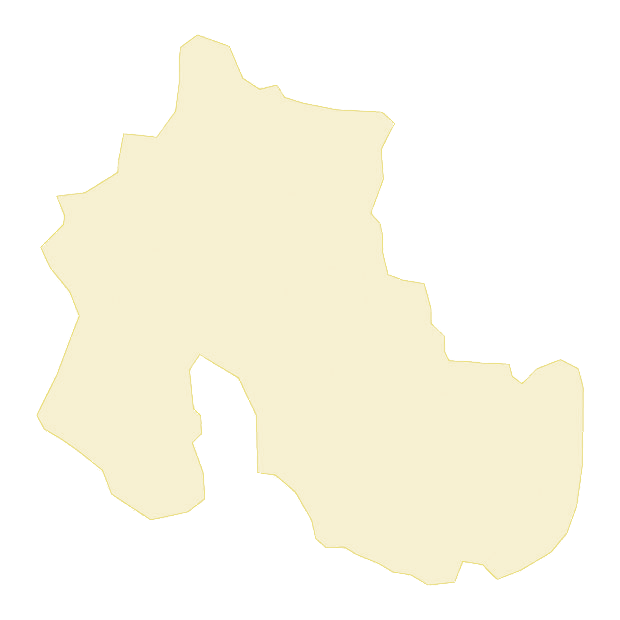
\includegraphics[width=0.95\textwidth]{../src/images/presentacion/jujuy.png}
%                 \caption{Frecuencia de uso en {Jujuy}}
%                 \label{fig:jujuy}
%             \end{figure} 
%         \end{column}
%     \end{columns}

% \end{frame}

